\documentclass{standalone}

% graphics
\usepackage{tikz}
\usepackage{pgfplots}
\usepackage{siunitx}

\begin{document}

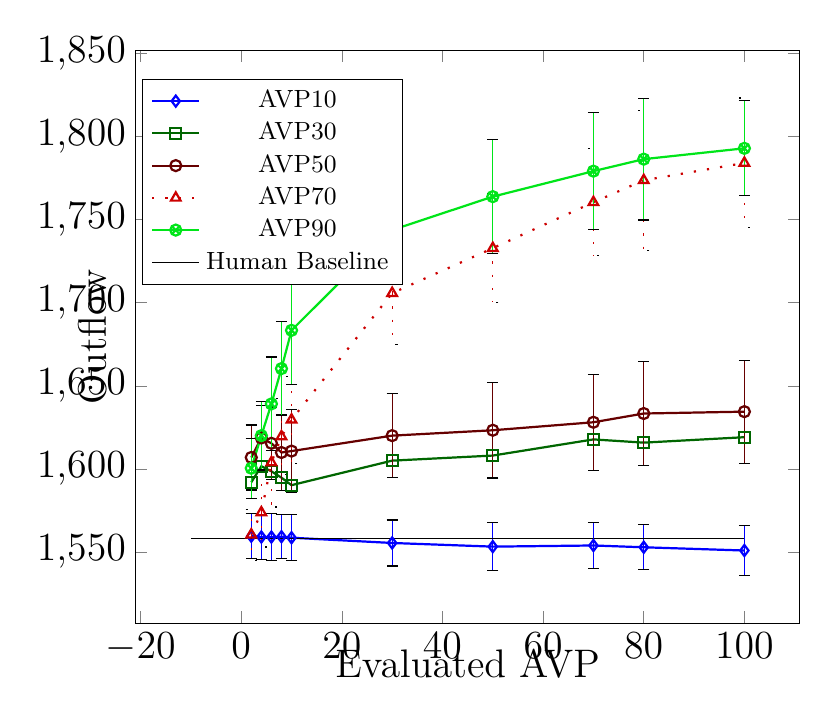
\begin{tikzpicture}[scale=1]
  \pgfplotsset{
      scale only axis,
      every x tick label/.append style={font=\Large},
      every y tick label/.append style={font=\Large},
	legend style={at={(0.01,0.95)},anchor=north west}
  }

\begin{axis}[
    legend style={font=\small},
	ylabel={\Large Outflow},
	x label style={at={(axis description cs:0.5,-0.03)},anchor=north},
	y label style={at={(axis description cs:-0.030,0.5)}, anchor=south},
	xlabel={\Large Evaluated AVP},
]




% trained on avp=10 
% dashdotdotted,
\addplot[mark=diamond, thick, mark options={solid, fill=blue!40, mark size=2 pt}, draw=blue, error bars/.cd, y dir=both, y explicit] table [x=a, y=b, y error=c] {
a	b   	c
2 1559.48 13.64
4 1558.98 13.35
6 1558.94 13.95
8 1559.16 13.39
10 1558.55 13.87
30 1555.38 13.85
50 1553.18 14.63
70 1553.87 13.93
80 1552.79 13.60
100 1550.84 14.98
};
\label{AVP10}

% trained on avp=30
% error bars/.cd, y dir=both, y explicit,
\addplot[mark=square, thick, mark options={solid, fill=green!60, mark size=2 pt}, draw=black!60!green] table [x=a, y=b] {
a	b   	c
2 1591.96 20.10
4 1601.57 21.10
6 1598.51 21.81
8 1594.69 19.23
10 1590.19 22.76
30 1604.95 24.25
50 1608.01 24.19
70 1617.73 29.72
80 1615.79 26.56
100 1619.06 28.24
};
\label{AVP30}  
%densely dashed, 
\addplot[mark=o, thick, mark options={solid, fill=black!60!red, mark size=2pt}, draw=black!60!red, error bars/.cd, y dir=both, y explicit] table [x=a, y=b, y error=c] {
a	b   	c
2 1606.86 19.58
4 1618.62 19.61
6 1615.39 21.84
8 1609.85 23.03
10 1610.71 24.87
30 1620.00 25.24
50 1623.24 28.74
70 1628.06 28.79
80 1633.32 31.13
100 1634.44 31.00
};
\label{AVP50}

%densely dashed, 
\addplot[mark=triangle, thick, loosely dotted, mark options={solid, fill=red!60, mark size=2pt}, draw=black!20!red, error bars/.cd, y dir=both, y explicit] table [x=a, y=b, y error=c] {
a	b   	c
2 1560.38 15.36
4 1573.70 20.76
6 1603.84 26.81
8 1619.50 23.10
10 1629.58 26.28
30 1705.79 30.68
50 1732.86 32.70
70 1760.51 32.22
80 1773.72 42.27
100 1784.16 39.10
};
\label{AVP70}

%densely dashed, 
\addplot[mark=otimes, thick, mark options={solid, fill=red!60, mark size=2pt},
draw=blue!10!green, error bars/.cd, y dir=both, y explicit] table [x=a, y=b, y error=c] {
a	b   	c
2 1600.38 18.04
4 1620.00 20.58
6 1639.12 28.21
8 1660.36 28.22
10 1683.40 32.37
30 1743.80 29.74
50 1763.89 34.40
70 1779.23 35.21
80 1786.46 36.61
100 1792.98 28.63
};
\label{AVP90}


%%densely dashed, 
%\addplot[mark=otimes, thick, mark options={solid, fill=blue!60, mark size=2pt},
%draw=blue!10!red, error bars/.cd, y dir=both, y explicit] table [x=a, y=b, y error=c] {
%a	b   	c
%2 1555.34 14.31
%4 1549.33 15.07
%6 1546.63 13.90
%8 1543.46 17.07
%10 1541.63 15.80
%20 1526.54 13.30
%30 1514.05 16.60
%40 1497.74 17.34
%50 1480.25 25.14
%60 1505.88 29.33
%70 1517.33 30.85
%80 1516.57 28.51
%100 1501.63 36.18
%};
%\label{linearPPO}

\addplot[mark=none, black, samples=200] coordinates {(-10,1558.12)
(100,1558.12)};
\label{Baseline}


\addlegendimage{/pgfplots/refstyle=AVP10}
\addlegendentry{AVP10}

\addlegendimage{/pgfplots/refstyle=AVP30}
\addlegendentry{AVP30}

\addlegendimage{/pgfplots/refstyle=AVP50}
\addlegendentry{AVP50}

\addlegendimage{/pgfplots/refstyle=AVP70}
\addlegendentry{AVP70}

\addlegendimage{/pgfplots/refstyle=AVP90}
\addlegendentry{AVP90}

%\addlegendimage{/pgfplots/refstyle=linearPPO}
%\addlegendentry{linearPPOAVP10}

\addlegendimage{/pgfplots/refstyle=Baseline}
\addlegendentry{Human Baseline}




\end{axis}
\end{tikzpicture}

\end{document}

